% Euclidean Handout Number Four
\documentclass{tufte-handout}

%\geometry{showframe}% for debugging purposes -- displays the margins

%%%% Packages to make things pretty
\usepackage{amsmath,amsthm}
\usepackage{booktabs}
\usepackage{graphicx}
\setkeys{Gin}{width=\linewidth,totalheight=\textheight,keepaspectratio}
\graphicspath{{graphics/}}
\usepackage{units}
\usepackage{fancyvrb}
\fvset{fontsize=\normalsize}
\usepackage{multicol}
\usepackage{pdfpages}

%%%% Theorem Environments
\theoremstyle{definition}
\swapnumbers
\newtheorem{problem}{Problem}[section]
\newtheorem{conjecture}[problem]{Conjecture}
\newtheorem*{definition}{Definition}
\newtheorem*{theorem}{Theorem}
\newtheorem{question}[problem]{Question}
\newtheorem{challenge}[problem]{Challenge}
\newtheorem*{postulate}{Postulate}

%%%%%


\title{Euclidean Geometry:\\An Introduction to Mathematical Work}
\author[]{Math 3600}
\date{Fall 2021} 

\begin{document}

\maketitle
\begin{marginfigure}
    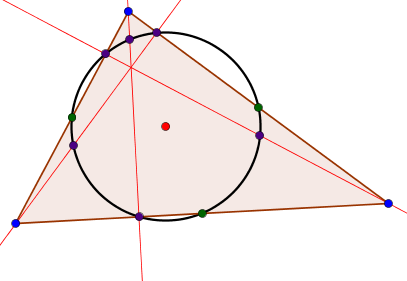
\includegraphics{NPC}
\end{marginfigure}

\setcounter{section}{4}
\section{Developing an Attitude of Skepticism}

I hope you have taken the time to look over the example paper by Professor Ball in Volume 0 of \emph{Transactions of Euclidean Geometry}.
One of our goals this semester is to develop a mathematician's healthy skepticism.
This can be a bit unsettling at first, but the basic idea is like a tee-shirt quotation: ``Question Authority."
Since this might be new to you, let me lead you a bit with the following items.

\begin{problem}\label{prob:Ball}
If you have not, yet, read Professor Ball's argument and figure out what went wrong.
Recall that you can find it in the public course folder under "Instructions for Authors".
Pinpoint his error and present it to the class.
\marginnote[-20pt]{Prof. Ball uses a result he calls the hypotenuse-leg theorem, which states that if two right triangles have two pairs of corresponding sides congruent, and one of the pairs is the hypotenuses, then the triangles are congruent. For now, we grant that this theorem is true, and is not the source of Prof. Ball's error. We'll come back to address this theorem later when we study triangles in detail.}
\end{problem}

Let's pretend that we overheard a tea-time conversation where a famous mathematician said, ``Sure Euclid's proof of I.7 is bad, but I can fix that.
It's proposition I.4 I'm worried about!"

\begin{problem}\label{prob:fix-I.7}
What might be the mysterious objection to Euclid's argument for Proposition I.7? Do you agree? If so, can you fix it?
\end{problem}

\begin{problem}\label{prob:fix-I.4}
What might be the mysterious objection to Euclid's argument for Proposition I.4? Do you agree? If so, can you fix it?
\end{problem}

So far, I have strongly hinted that the arguments for Propositions I.1, I.4 and I.7 have sometimes been judged as imperfect in some way.
Unfortunately, they are not alone.

\begin{problem}[Standing Problem]
As the semester progresses, we will have occasion to read over a hundred different arguments by Euclid, if any of the others we read have gaps, please consider giving a short presentation about it.
(Hint: there are several of these to be found.)
\end{problem}

The big lesson here is that \emph{The Elements} is not perfect, from a modern point of view.
This worried mathematicians for a long time, and it took two millennia until all of the issues were finally sorted out to the community's general satisfaction.
Several re-axiomatizations of planar geometry have been proposed, the most famous versions are due to David Hilbert, George Birkhoff, and The School Mathematics Study Group.

\vfill
\end{document}